\documentclass[10pt,a4paper]{article}
\usepackage[margin=2.2cm]{geometry}
\usepackage{fontspec}
\usepackage{kotex}
\setmainfont{Apple SD Gothic Neo}
\setsansfont{Apple SD Gothic Neo}
\usepackage{amsmath,amssymb}
\usepackage{graphicx}
\usepackage{caption}
\usepackage[dvipsnames]{xcolor}
\usepackage[colorlinks=true,linkcolor=MidnightBlue,citecolor=MidnightBlue,
            urlcolor=MidnightBlue]{hyperref}
\usepackage{titlesec}
\titleformat{\section}{\large\bfseries}{\thesection}{0.6em}{}
\captionsetup{font=small,labelfont=bf}
\setlength{\parskip}{0.35em}
\setlength{\parindent}{0pt}
\usepackage{mdframed}
\newmdenv[linewidth=0.4pt,linecolor=gray!60,backgroundcolor=gray!5,
          innertopmargin=6pt,innerbottommargin=6pt,skipabove=8pt,skipbelow=8pt]{claimbox}
\newcommand{\claim}[2]{\begin{claimbox}\textbf{주장.} #1\par\smallskip
  \textcolor{gray!70}{\textbf{반증 조건.} #2}\end{claimbox}}

\title{\bfseries 홑 봉인은 판정하지 못한다\\[2pt]
\large 그리고 결측선의 절반은 우리 손이 그었다 --- 수확 자 완결(리허설 $2$)}
\author{월드모델 실험실 · 노트 $846$}
\date{2026-08-08}
\begin{document}\maketitle

\section{한 줄}

$845$ 가 남긴 세 구멍(합성 밴드 부재 · `한 축' 무해부 · 결측의 정체)을 티처
\#$12$ 가 찔렀고, $8/12$ 첫 라벨 관측 전의 청정 창 안에서 전부 쟀다. 결과:
결측 하락과 $m{=}30$ 뽑기 요동을 같이 얹은 \textbf{합성 밴드가 $0.209 \pm
0.357$($2\sigma$)} --- 동결 문턱 $0.2046$ 이 밴드 속에 잠긴다. \textbf{봉인
$1$호 하나로는 아무것도 재판정할 수 없다}(`총붕괴 아님/보류'만) --- 전향
판정은 봉인 누적($\ge 60$편) 전용으로 강등.

\begin{figure}[t]\centering
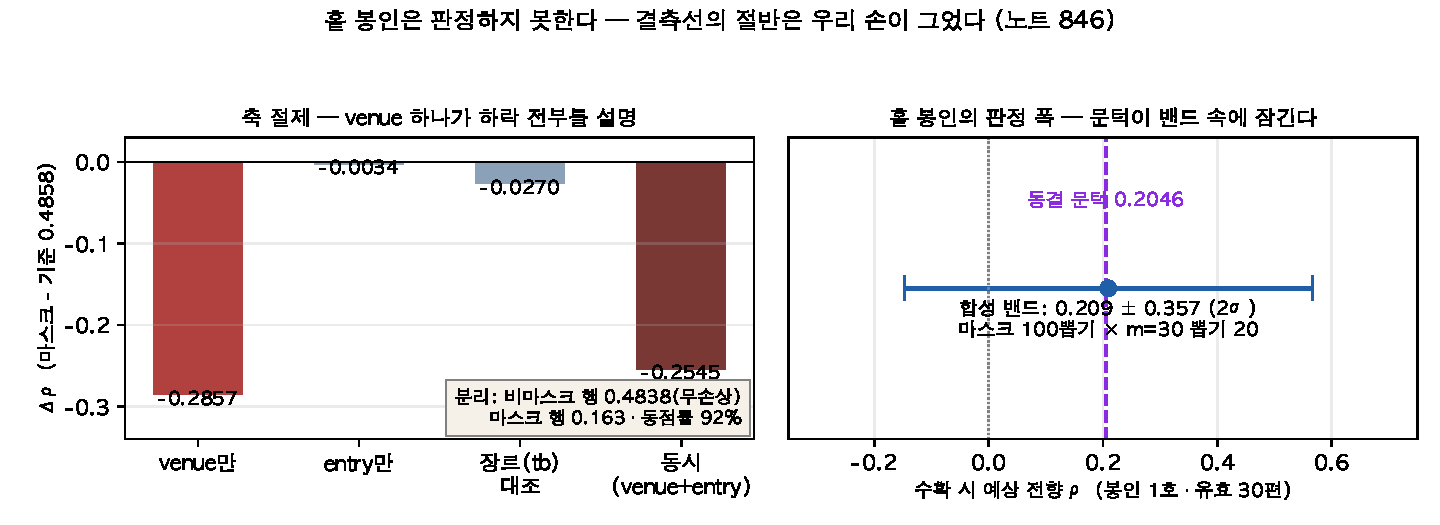
\includegraphics[width=0.97\textwidth]{figs/halfline.pdf}
\caption{왼쪽: 축 절제 --- venue 단독 $\Delta{-}0.286$ 이 동시 마스크
$-0.254$ 를 단독으로 다 설명한다. 오른쪽: 합성 밴드와 문턱.}
\end{figure}

\claim{\textbf{`영화 신호는 배급 축 하나'가 이번엔 추론이 아니라 절제로
확정됐다.} venue 만 $\Delta{-}0.2857$ · entry 만 $-0.0034$ · 장르 대조
$-0.027$. 분리 채점이 기제까지 보였다: \textbf{비마스크 행 $\rho$ $0.4838$
(기준 $0.4858$ 에서 무손상) 대 마스크 행 $0.163$ 붕괴 · 마스크 행 동점률
$92.3\%$} --- 모형 취약이 아니라 정보 소실이고, $0.5$ 로 뭉친 행들끼리
판별이 소멸하는 동점 압축이다. 그리고 결측 부검: 봉인 $13$편 중
\textbf{버그류 $7$}(휴리스틱 · 손 검증 확정 $3$ --- `이화배컴퍼니(주)' 는
사전에 정확히 있는데 공동배급 연결 문자열이 놓쳤다) · 사전 밖 $5$ · 원문
없음 $1$. \textbf{결측선의 절반가량은 코드가 그은 선이다} $\to$ 별칭 정규화
v$2$ 를 봉인 $2$호 \emph{전} 동결로 격상 --- v$1$ 정본 + v$2$ 보조 두 벌
봉인이면 `결측선' 진단이 전향 시험으로 바뀐다.}
{합성 $2\sigma < 0.35$ 였다면 홑 봉인 판정은 살았다(실측 $0.357$ 로 사망).
venue 단독이 전체의 $80\%$ 미만이었다면 `한 축' 은 철회됐다(실측 $112\%$).}

\section{정직 --- 그리고 예측 채점 $6/6$}

부검 $7$ 은 토큰 부분일치 휴리스틱의 상한 쪽 추정이다(손 확정 $3$). 마스크
기제는 여전히 무작위 근사(봉인 결측은 소형 편향)다 --- 분리 $\rho$ 가 그
부담을 줄였을 뿐이다. 이번 사이클은 $3$연속 크기 미스의 교훈대로 \textbf{크기
예측을 버리고 순서·문턱 주장만 걸었고 $6/6$ 전부 맞았다} --- 예측의 격을
낮추니 적중이 돌아왔다. GitHub 흐름 $8$회째(이슈 \#$18 \to$ PR \#$19$).
판 $\rho$ $0.4710$ 그대로.

\end{document}
